\documentclass[a4paper,fleqn]{cas-dc}
\usepackage[numbers]{natbib}

\setcounter{figure}{0}
\usepackage{tabularx}
\usepackage{mathtools}
\usepackage{booktabs}
\usepackage{pgfplots}
\usepackage{flushend}
\usepackage{float}
\usepackage{graphicx}
\usepackage{algorithm}
\usepackage{algorithmic}
\usepackage{amsmath}
\usepackage{amssymb}  % Add this for \mathbb
\usepackage{tikz}
\usepackage{subcaption}

\numberwithin{equation}{section}

\begin{document}
\let\WriteBookmarks\relax
\def\floatpagepagefraction{1}
\def\textpagefraction{.001}

\shorttitle{GNN using Iot}
\shortauthors{S Gopikrishnan et~al.}

\title [mode = title]{Graph Neural Network-Driven Routing Intelligence for Large-Scale IoT}                      
% Name : BEERALA DINESH
%Reg No : 23MIS7217
%gmail : veerudinesh7405@gmail.com
%vit ap mail : dinesh.23mis7217@vitapstudent.ac.in
%orc id : 0009-0000-1323-0129

\author[1]{B Dinesh}[orcid=0009-0000-1323-0129]
\ead{dinesh.23mis7217@vitapstudent.ac.in}
\address[1]{School of Computer Science and Engineering, VIT-AP University, Amaravathi. Andhra Pradesh, India}


\author[1]{Author-2} [orcid=0000-0001-9082-9012]
\cormark[1]
\ead{gopikrishnan.s@vitap.ac.in}


\author[3]{Author-3} [orcid=0000-0001-9082-9012]
\ead{gopikrishnan.s@vitap.ac.in}


\cortext[cor1]{Corresponding author}

\begin{abstract}
The growing proliferation of devices on the Internet of Things (IoT) has made modern networks increasingly vulnerable to sophisticated cyber threats. Traditional intrusion detection systems (IDS) struggle to maintain high detection accuracy in the presence of high-dimensional data and extreme class imbalance, particularly for rare but critical attacks. The growing proliferation of devices on the Internet of Things (IoT) has made modern networks increasingly vulnerable to sophisticated cyber threats. Traditional intrusion detection systems (IDS) struggle to maintain high detection accuracy in the presence of high-dimensional data and extreme class imbalance, particularly for rare but critical attacks. The growing proliferation of devices on the Internet of Things (IoT) has made modern networks increasingly vulnerable to sophisticated cyber threats. Traditional intrusion detection systems (IDS) struggle to maintain high detection accuracy in the presence of high-dimensional data and extreme class imbalance, particularly for rare but critical attacks. The growing proliferation of devices on the Internet of Things (IoT) has made modern networks increasingly vulnerable to sophisticated cyber threats. Traditional intrusion detection systems (IDS) struggle to maintain high detection accuracy in the presence of high-dimensional data and extreme class imbalance, particularly for rare but critical attacks. The growing proliferation of devices on the Internet of Things (IoT) has made modern networks increasingly vulnerable to sophisticated cyber threats. Traditional intrusion detection systems (IDS) struggle to maintain high detection accuracy in the presence of high-dimensional data and extreme class imbalance, particularly for rare but critical attacks.
\end{abstract}

\begin{keywords}
Intrusion Detection System (IDS) \sep 
Internet of Things (IoT) \sep 
Class Imbalance \sep 
Feature Selection \sep
Deep Learning \sep 
Convolutional neural networks (CNN) \sep
Data Augmentation
\end{keywords}


\maketitle



\section{Introduction}
However, complexity has emerged within the options in terms of routing and managing the flow of traffic of the proposed communication networks in the next generation of communication networks, i.e., in IoTs, WSNs, software-defined network communication technologies, and related smart grid communication technologies. Besides the aforementioned communication networks in communication networks, complexity in terms of the impact of energy constraints on communication networks has added more complexity in terms of managing and routing alternatives proposed by these communication networks.



Apart from this, recent developments in Artificial Intelligence have led to the development of intelligent optimization techniques for the entire network using Graph Neural Networks (GNN). It would also help to mimic the real-world graph on the network. Deep Reinforcement Learning (DRL) would help in developing adaptive processes on the networks by interacting in real-time. GNN would also help in developing more intelligent routing on the network with the help of DRL; this would also be more relevant in terms of scalability.



Furthermore, it is analyzed that the developed intelligent methods are restricted with reference to the perplexity of various factors such as scalability, intelligence.
\subsection{Background and Context}
Contemporary communication networks, e.g., software networks, smart grids, and large-scale traffic engineering networks, are facing an even more problematic dynamic nature of traffic, network performance requirements, and the complex requirements constituted in the innumerable criteria. The other recent papers have revealed that the Graph Neural Networks (GNNs) possess significant potentials in helping to develop a wide range of communication networks by capturing topological properties, traffic patterns, and other resource restrictions within a communication infrastructure of network establishment by illustrating the possibilities of traffic engineering, as shown by MAGNNETO and G-Routing, the SDN-based proactive model of traffic engineering uses Deep Q-Network and Graph Neural Networks to substantially enhance fault tolerance, against the conventional methods which only help to promote QoE by propag.

\subsection{Research Opportunities}
Although, of course, these solutions in this specific sphere in modern times are quite prospective, nevertheless, gaps exist, and this specific sphere of multisagents GNNs in a concrete environment of specific scalability ought to be researched. Moreover, a specific problem, namely, a question of a possibility to solve this specific optimization problem while taking into account a wide range of time constraints, a question of reliability, a question of conggesting, a question of efficiency in a specific case of a specific question of routing efficiency while maintaining reliable quality has not been studied in sufficient detail. Secondly, a specific question of efficiency in this specific environment while maintaining a centralized model in a specific case while quality in this specific sphere is of sufficient value has not been studied in sufficient detail. Thirdly, a specific question of a possibility to solve a specific question of applying an online learning model while relying upon a specific question of a so-called federative learning model in a specific question of applying this model in this specific sphere while maintaining a specific question of minimization of a cost related to a specific question of efficiency of this model in this specific sphere has remained.
\section{Research Objectives}
\paragraph{Objective 1}
\cite{Bernardez2023494,Li2025}
aimed to develop a new paradigm for routing in large scale IoT networks by employing Graph Neural Networks (GNNs) and considering dynamic graphs as network topologies which they they learn to route within their context. This goal seeks the deep learning-based solution to the problem of determining meaningful representations for message-passing operations on graphs over nodes, links, and traffic states. It is an alternative to traditional methods that use predefined metrics and operate in a localized manner.

\paragraph{Objective 2}
\cite{Islam2024111169,Pehlivan2025}
The main purpose of this paper is to describe an algorithm that seeks to learn a routing policy and can improve itself by learning some given techniques via Graph Neural Networks. This algorithm will intentionally focus on the most crucial QoS parameters for which we believe could offer better solutions if reducing delay, congestion avoidance, packet loss prevention and energy usage consumption and finally make networks intelligent to handle traffic load fluctuations over time and space in large scale IOT deployment system.

\paragraph{Objective 3}
\cite{Das2025204}
This will be accomplished by enhancing the learning process in the creation of intelligent IoT routing, so that the suggested method can function effectively even in situations where topology changes, traffic fluctuations, and/or network failures occur. In particular, this goal inquires as to whether the learned routing policy can be applied to unknown network configurations without sacrificing consistent high performance in extremely dynamic and diverse IoT environments.

\paragraph{Objective 4}
\cite{Wei202390}
to assess the effectiveness of the suggested GNN-driven routing strategy using in-depth simulations and a comparison with both conventional and cutting-edge routing protocols. To show the efficacy and viability of the suggested solution for large-scale IoT networks, the evaluation will take into account metrics like end-to-end latency, packet delivery ratio, energy efficiency, routing overhead, and scalability.

\section{Literature survey}
\subsection{Deep Reinforcement Learning and Graph-Based Routing Optimization for Next-Generation Networks}
This paper \cite{Suresh2024} shows Intelligent data routing strategy based on federated deep reinforcement
learning for IOT-enabled wireless sensor networks  how to guide traffic through a network - letting every switch teach itself then swap only the lessons, not the raw messages. Because no private details ever leave the machine where they were first seen, the scheme fits networks that are spread far apart. The benefit is clear - secret payloads stay on their home devices but the whole network still figures out the smartest next hop. It also grows without trouble as more switches join. The trade off is that learning takes longer, because news about good moves travels only through summaries and chatter among the switches adds extra load, above all when links flicker.

The study \cite{Yu20238806} presents a deep reinforcement learning method that chooses routes and sending moments for traffic of mixed importance, where some data streams carry more weight than others. The model learns how to steer packets plus set their departure times so that the most urgent traffic meets its tight deadlines while the remaining traffic is still delivered without needless delay. A plain advantage is that life critical applications receive their data on a steady, predictable schedule. But training the model calls for lengthy runs and careful adjustment. The system also relies on powerful hardware but also exact knowledge of the traffic pattern, two requirements that limit its use in networks where resources are scarce.

This paper \cite{Jiang2024} shows how graph neural networks improve routing - treating any network as a plain map of points and lines. A GNN learns how those points plus lines interact and keeps up when the map changes. It sees what happens next door and across the whole map at once - it picks better paths. The price is heavy arithmetic but also long training runs on big maps. Once trained, the net is hard to read - spotting a fault or putting it on live gear is slow work.

This paper \cite{LuSDN2025} explains graph neural networks and their application in many different industries including telecommunications, manufacturing, energy systems, and transportation. GNNs have an advantage in being able to process data with complex relationships and that have irregular structures. GNNs provide an extremely accurate solution to real-world problems and have a very high ability to learn through generalization of experience. The examples shown in this paper of GNN’s being used within the industry will show GNN’s outperforming all methods currently being used. However, the paper also points out some major challenges to the adoption of GNNs, including the need for large datasets that have been marked or tagged by humans, the high computational costs associated with using these networks, and the difficulty associated with real-time deployment of GNNs. These challenges will probably impede the continued use of GNNs, especially in industries that must make quick decisions based upon minimal time delay between data acquisition and resulting decision-making.

The article \cite{Devika20241329} presents a novel routing approach of WSNs by way of integrating DQRL with Butterfly Optimization Algorithm (BOA) originated by the MOD-LEACH route. The overall objective of this route algorithm is to minimize the energy used by WSNs and maximize WSN lifetime. The route algorithm utilizes the state of the WSNs at that moment to facilitate in the choice of route between balanced routes of WSNs or to find the optimal CHs to every WSN. In addition to the enhanced WSN route algorithm to ensure greater energy efficiencies in the networks and less packets being lost in the networks to ensure greater stability in the functioning of the networks by ensuring greater services of WSNs through greater energy efficiencies, increased system complexity will be realized as opposed to the case of BOA. Therefore sensor networks implementation will face more challenge than the case of BOA.

In this study,\cite{Logeshwaran2024} a hybrid optimization framework is introduced which can be employed to manage the large IoT traffic in the 6G networks in the future. The mechanism uses smart multi routing mode to distribute the traffic to over a single route and the congestion is reduced and the performance of the entire network is better. Among such advantages is enhanced reliability, lower latency and enhanced control of dense IoT landscapes. The system can also be scaled to support the dynamic traffic requirements hence it is the appropriate system to implement in the next generation networks. However, additional control and signaling overhead are generated by the method. Moreover, it needs very fine network state information, not always provided, which complicates and increases the cost to operate on a large scale in 6G IoT networks.
\begin{table*}[t]
\centering
\caption{Comparison of GNN-Based Routing Techniques for IoT Networks}
\renewcommand{\arraystretch}{1.25}
\setlength{\tabcolsep}{5pt}
\begin{tabular}{|p{0.06\textwidth}|p{0.20\textwidth}|p{0.22\textwidth}|p{0.22\textwidth}|p{0.22\textwidth}|}
\hline
\textbf{Ref} & \textbf{Method Proposed} & \textbf{Techniques Used} & \textbf{Issue Resolved} & \textbf{Limitations} \\
\hline

\textbf{[\cite{Mohan2025}]} &
Intrusion detection pipeline for WSNs where a GNN model is tuned using an Osprey-inspired optimizer. &
Osprey Optimization (metaheuristic) for feature/hyperparameter search; GNN to capture node-link dependencies in traffic. &
Boosts attack detection by exploiting relational patterns in sensor communications and improving model settings automatically. &
Optimization search can take many iterations; GNNs may be too heavy for tiny sensor hardware; results can drop if the attack dataset is small or not representative. \\
\hline

\textbf{[\cite{Thakur2025}]} &
A literature review that organizes AI-based energy-aware routing ideas for IoT-WSNs rather than proposing a single new protocol. &
Survey of ML, DL, and RL routing; clustering, duty-cycling, and heuristic optimizers; comparison of metrics and test setups. &
Clarifies which AI choices help reduce energy use and extend lifetime, and highlights common evaluation practices and gaps. &
No new algorithm to reproduce; findings depend on included studies; real deployments may behave differently than simulation-heavy benchmarks. \\
\hline

\textbf{[\cite{Jiang2025}]} &
Riskquant-GRL: graph deep RL control approach for communication decisions in power network settings with risk-aware rewards. &
Graph state encoding of grid/comm topology; deep RL policy learning; variance- or risk-sensitive reward shaping. &
Improves self-optimizing control by balancing performance with reliability/risk considerations in critical power communications. &
Training can be data- and compute-hungry; reward design is delicate; safe exploration is hard in critical systems without high-fidelity simulators. \\
\hline

\textbf{[\cite{Lee2025}]} &
Routing optimization method for 6G where node embeddings guide a genetic algorithm toward better candidate paths. &
Graph/feature embeddings; GA operators (selection, crossover, mutation) for multiobjective route search. &
Speeds up route discovery and improves QoS objectives by using embeddings as “hints” to steer the GA search. &
GA still scales poorly for huge topologies; embeddings can become outdated when links change fast; tuning GA parameters affects repeatability. \\
\hline

\textbf{[\cite{Kavitha20251463}]} &
Energy-aware clustering scheme that combines Firefly global search with Gradient Descent refinement to select cluster structures. &
Firefly Algorithm for exploration; Gradient Descent for local improvement; clustering and cluster-head selection logic. &
Reduces energy drain and balances load by improving cluster-head placement and cluster formation, extending network lifetime. &
Hybrid steps add overhead; convergence depends on step sizes and firefly parameters; may rely on simplified radio/energy assumptions. \\
\hline

\textbf{[\cite{Kaal2025427}]} &
Adaptive microgrid optimization framework using a DRL--GNN model plus dynamic clustering to coordinate multi-energy assets. &
GNN for topology/state representation; deep RL for sequential decision-making; dynamic clustering of sources/loads. &
Handles changing demand and supply by learning coordinated control strategies that improve overall efficiency and stability. &
Needs extensive training and realistic simulators; explainability is limited; deploying learned policies safely in real grids is non-trivial. \\
\hline

\textbf{[\cite{Eldho2025614}]} &
Reliability and fault detection model for WSN-assisted autonomous vehicle systems using QHHO to tune a GNN-based predictor. &
(Quantum) Harris Hawks Optimization for tuning/feature selection; GNN for relational fault inference and reliability scoring. &
Detects faults earlier and evaluates reliability by modeling interactions among sensor nodes and communication links. &
May be heavy for real-time vehicle pipelines; optimization adds runtime/training cost; generalization can weaken across new routes, weather, or hardware. \\
\hline

\textbf{[\cite{Karthikeyan2025}]} &
Selective GCN routing approach that processes only the most relevant parts of the network graph to reduce cost. &
Graph Convolutional Network; selective neighborhood/subgraph filtering (attention-like gating) for efficiency. &
Cuts routing computation while staying topology-aware, enabling faster decisions than full-graph processing in many cases. &
If selection misses key nodes/links, decisions degrade; still requires good graph features; dynamic conditions can break assumptions about “relevant” subgraphs. \\
\hline

\hline
\end{tabular}
\end{table*}
\subsection{Graph-Based and Software-Defined Approaches for Energy Efficiency, Reliability, and Traffic Management in IoT and WSNs}
This review paper \cite{Isyaku2024} discusses several software-defined networking based routing solutions that can be considered to load balance the wireless sensor networks in internet of things applications. SDN enables decision-making and the management of resources in a centralized manner by separating control plane and data plane. Its key benefit is enhanced flexibility, simplified network administration, and traffic optimization. Another aspect that the review covers is the fact that SDN provides faster response to changes in the network. Scalability problems and single point failures are challenges however brought about by centralization. Regular contact with the controller is also liable to add latency and energy usage which is a significant disadvantage to energy constrained sensor and IoT networks.

This literature review article \cite{Ferrer-Cid2025} reviews various graph solution techniques developed and used to ensure quality in data collected using IoT sensors within a monitoring network. Relations between sensors are examined and represented in graphical models to identify faulty sensors, loss of data readings, and anomalies within data collected. Firstly, higher accuracy and reliability of data collected from sensors resulting in a boost in network and decision-making performances constitute a benefit. Additionally, advanced defect detection and analysis can be performed with a graphical technique. Another disadvantage relates to memory and computation, which within graphical solutions, can be intensive. Scheduling sensors involving a large number of sensors within a real-time system may be difficult, particularly involving data value fluctuations and limitations of sensors within a system.

In this article \cite{Lu2025}, a graph based reinforcement learning framework is proposed. Based on the graph representation of the network topology, the algorithm generates optimal traffic control strategies based on the network. The proposed framework has benefits in terms of improved load balance and congestion relief in the network. Also, traffic control in the network can be adapted dynamically. The proposed framework has a disadvantage in that the learning process may be unstable. Also, computational costs may be involved in the stability of the learning process. The framework may have difficulties in implementing large-scale networks.

This paper \cite{BlessinaPreethi20253320} proposes a hybrid solution by employing Knowledge Graph Neural Networks and the Analytic Hierarchy Process to enhance the sustainability within the wireless sensor networks. This solution is ideal for intelligent routing and resource management, incorporating various factors such as the level of energy and priority nodes. The major benefit offered by this solution is the increased lifetime and balance in energy usage among the static nodes. The hybrid model is however complex and requires heavy computation. This solution may not easily be implemented within the low-cost wireless sensors.

In this paper,\cite{Arulanandam2025} a hybrid approach of multi-objective learning, and Artificial Rabbits Optimization technique and mutation operations is presented in order to introduce a cluster-based routing method of wireless sensor networks. Concisely, it tries to prefer superior cluster members, superior routes, in the light of multiple conflicting needs, which include energy consumption, network life, and communication performance. Conversely, the method is more advantageous since clustering is normally considered to reduce waste of energy and multi-objective optimization is capable of ruling out the possibility of the existence of such alternatives, which are optimal in one objective but poor in one objective, as it is commonly termed as Pareto optimal. Conversely, another disadvantage of this method is complexity since the process is a combination of learning with perturbation, mutation as well as metaheuristic optimization.

This current study \cite{Zoican2024} will present a model using graph neural networks in traffic prediction, but this one will be optimized to be executed using microcontrollers, which has low computing power. This will entail using the idea of graph structure to design road infrastructure and thereby predict traffic movement without having to consider cloud computing to a large extent. This will be a benefit since it will be energy-efficient and allow predictions to be done to reduce delays and bandwidth consumption. This current idea can also apply to a smart city setting, which will require rapid predictions by sensors. This model will be a con since microcontrollers will be limited in terms of memory and ability to compute. Thus, it appears that this current idea will most probably be optimized or pruned. Another notion will be in regards to training models, which will not be applicable to be used in a microcontroller compared to using a central server.

This systematic review\cite{Liu2025164883} examines the applications of graph neural networks for assessing the reliability and resilience of infrastructure networks such as power, transportation, and water networks. Because these networks have inherently graph structures, graph neural networks are able to discover patterns associated with network failure, network recovery, and vulnerabilities of the graph. Additionally, the benefit of graph neural networks in this respect is that it can model intricate dependences that are difficult for most models to approximate, particularly for failures that are distributed in linked components of the network. On the other hand, some of the demerits of graph neural networks include the fact that they are computationally expensive, and often, large amounts of data are required for training. Lastly, the disadvantage of these networks is that it is difficult for them to provide explainability, especially for networks like power, which are concerned with safety and security.
\subsection{Advanced Graph Neural Network Models and Emerging Applications in Next-Generation Intelligent Networks}
This research \cite{Wang2025} presents GATR, an approach for optimizing the RPL routing protocol, which can be used for both IoT networks and low power loss networks, using the Graph Attention Network and Deep Reinforcement Learning. Also, graph attention mechanisms of GATR enable attention to focus on the most prominent nodes and edges, whereas deep reinforcement learning enables training of the system for learning of the decision depending upon the results of trials and errors. In addition, there has been the development of the variance-sensitive reward system. There are controls for dealing with the volatility of performances, and there is the penalty for risky and irregular routing, which enables improving the robustness of routing towards changes over time. Some of the most critical advantages of GATR are its superiority over current approaches for improving the quality of routing, changes in the network, and stable learning of rewards with the reinforced learning approach. However, GATR presents high training overhead and high costs. Some examples of convergence of the model may be unstable and slow.



This research article \cite{Shi2025} addresses an issue connected with entity alignment, a process of aligning entities of a common real-world object represented in two different graphs of knowledge (e.g., “New York City” entities in two datasets). This research, named RRDGNN, relies on both relation and reflect learning and attempts to untangle various kinds of information to make it possible to accurately match entities, even if graphs contain many noises or missing information. Strengths of using such a model include untangling relations, which could make it possible to unconfuse similar entities, thus improving accuracy during domain alignment. Weaknesses of such a model include that they can be computationally intensive and difficult to learn, especially if they include large graphs.

The currently proposed study \cite{Manikantha20251031} introduces a new routing mechanism for smart device networks (Internet of Things [IoT]) using a new method consisting of multilayer clustering combined with deep learning to reduce the amount of energy utilized. By the nature of the multilayer clustering method, devices will be arranged in a hierarchical manner to enable more efficient organization of all communications while utilizing the deep learned intelligence from the network to make routing and cluster-head decisions much more efficiently than traditional methods (rules). The main advantages to this approach are that it will provide greater energy conservation and greater lifetime usage of battery-powered devices, plus improved scalability, particularly in larger density smart device (IoT) networks. The new method will be adaptable to constant changes experienced in large density device networks. However, there are several disadvantages to the method, the most significant being that deep learning requires greater computational resources to implement than rules and that the data needed to train the deep learning architecture could be very difficult to source or compile in real-world situations; as such, deep learning may produce poor results if trained to work in a specific context but then applied in a different context. Also, problems can exist with clusters when cluster heads fail or the cluster is subjected to excessive processing loads.

This paper \cite{Ali202585447} presents innovative techniques for topology optimization using the combination of deep reinforcement learning and graph neural networks. Topology optimization involves the identification of the best placement and movement of nodes and links that maximize or optimize performance, robustness, and cost savings. Graph neural networks are efficient tools for representing network topology, and deep reinforcement learning algorithms learn how to adjust and/or choose network topology to meet certain goals such as delay minimization and throughput maximization. The combination of both techniques offers greater effectiveness and adaptability in modifying and evolving network topology for complex networks that are difficult to handle using traditional techniques. However, adjustments of network topology could be very expensive and unrealistic in real systems for various reasons, as not all links and wires are adjustable and easy to manipulate. Additionally, the process of training these algorithms involves significant simulations that may lead to sensitive results depending on certain assumptions.

This review \cite{KrishnaMoorthy20261803} discusses the current state of applications of graph neural networks (GNNs) in both IoT and NextG networks, and it includes applications such as routing, traffic prediction, security, fault detection, and resource allocation. It also explains the relevance of GNNs and why current applications of graph structures are best suited for the technology. Indeed, one of the benefits of this review is that it enables the reader to easily grasp the overall state-of-the-art of applications of GNNs and make comparisons between various approaches. The cons of this review are essentially related to the technology being discussed, and these include that GNN applications are computationally expensive and that GNN applications and results have not been validated under real-world conditions since most of these applications are simulated.

The article \cite{XuanTung20262226} will focus on the recent trends in the application of the graph neural networks in the next-generation IoT networks, among other issues that are yet to be resolved. It is most likely that the paper will refer to the latest advances in the application of different versions of GNNs to facilitate topology-driven learning, dynamic routing, collaborative devices, and secure networks. The advantage of the paper is that it offers an up to date opinion on the use of graph neural networks in improving the IoT intelligence, particularly in intricate IoTs. Its disadvantage is that graph structures in most graph neural network solutions must be more or less precise, whereas, with IoT networks, the network connections may be unreliable or may be dynamic most of the time. The other factor is in scaling up the graph neural network solutions that can occasionally be supported in edge computing or in cloud computing.

This article\cite{Binshaflout2026}  is a review of graph neural networks in vehicular social networks in which cars not only interact with each other in location-based interactions but in social-like ways too, such as going through the same paths, having the same interest, or behaving in the same manner. The graph neural networks are based on vehicle-to-vehicle interaction and improve activities such as message dissemination, identification of trust models, traffic forecasting, and anomaly identification. The benefit of doing so relies on the fact that this method would be capable of acquiring both the mobility model and structure information regarding relationships, improving the quality of forecast to make decisions in a significantly enhanced manner. The disadvantage is severe in reality. Firstly, vehicular networks are always varying in a highly dynamic manner at a tremendous speed. Graph structure also gets outdated soon. Privacy and security are also prime considerations since social relationships may lead to exposure of sensitive behavior patterns. The next consideration is computation cost in real-time decision-making.


\subsection{Research gaps}
This may be the case in the current state of affairs.. There is one more thing to consider. The research has a lot of gaps on the trends. The reason is that there are numerous problems in the current trends that are yet to be resolved. The things are related to the current trends and that is why these issues are not disappearing. The issues associated with the current trends are very difficult to resolve. It is actually the Internet of Things networks that this research is examining. It is scouting sections of the Internet of Things networks. Such networks possess items that never change such as the way they are configured and their sizes. This matters in case we consider the traffic flow in the Internet of Things networks.

This will have an impact on the effectiveness of this research in all types of Internet of Things networks. Internet of Things networks are quite dissimilar. Are used in a number of ways. We should consider whether this research will be effective with all of them. We would like to ensure that it is Internet of Things networks, in general. GNN considering its features of being able to guarantee routing in terms of network situations as regards scalability would also entail a significant portion as a constraint in terms of how such an issue would also be entrenched in a specific sense in terms of being able to make sure there are capabilities.
\subsection{Motivation}
There are many reasons why this research was needed; one of them is the complexity that has characterized contemporary and emerging internet of things and network technologies. There are billions of interconnected and intelligent devices that generate dynamic and heterogeneous network activities. Due to this increased complexity, contemporary and heuristic-based network protocols and algorithms cannot provide network operations that meet required and stringent network and performance demands. According to this research, one of the reasons that prompt the development of intelligent and adaptive network routing protocols and algorithms was to take advantage of the advanced and increased capacity to represent and analyze the network connectivity and intelligent relationship by Graph Neural Networks and to utilize the advanced ability of Deep Reinforcement Learning in order to interact and adapt to network environments.
\subsection{problem statement}
The main problem in this research is trying to solve is that to develop a routing mechanism for large IoT networks that have highly dynamic topologies with varying amount of traffic. Traditional routing schemes do not have adequate performance when there are several objectives that have to be satisfied. This is particularly valid when there is failure within the overall topology of these scenarios. There is a requirement for learning mechanisms such as GNN-based and DRL-based solutions because they appear to have adequate performance. However, when implemented within a real-world application, they have poor performance. They do not have sufficient ability to generalize, they have high computing power consumption, and they have weak performance that is not sufficient. The overall requirement is to recognize which of these GNN-based routing mechanisms is capable of determining what is of primary importance within the overall network and making adequate routing decisions with high efficiency while at the same time performing well.

\section{Proposed Methodology}
\subsection{Proposed Framework}
In this paper, an intelligent routing approach for large-scale IoT networks by employing the use of Graph Neural Networks (GNN) combined with the adaptive learning approach is proposed. In the presented method, first, a network graph is generated in which the nodes of the graph include the sensor nodes and the connections between these nodes form the edges of the graph. Then, at each time step, every node collects the network information like traffic load, remaining energy of the nodes, delay and quality of the links that are regarded as the dynamic states of the network. Moreover, preprocessing of the gathered information is done to generate feature vectors as input data for the GNN model.

The next step in this framework includes running the model on the prepared dataset. In contrast to the classical methods in routing schemes that are based on the static measurements and use shortest path algorithm, the GNN model is trained based on the dynamic states of the network. Therefore, in addition to the shortest route selection, considering other important criteria like congestion avoidance and energy efficiency becomes possible by means of the proposed approach.

Finally, in this approach, a decision-making module should be designed to determine the optimal paths based on the training of the GNN. Moreover, as another module of the framework, a feedback loop is designed that monitors the parameters like throughput, packet delivery ratio, delay and energy consumption and consequently adapts the model to changing network conditions.
The suggested framework would be created to act as a distributed intelligent routing system, which would continuously evolve depending on the changes happening in the network and experience gained from past interactions. Contrary to traditional routing techniques that work based on predefined settings and/or scheduled updates, the suggested model will allow the system to make decisions at any moment by implementing data intelligence within the network layer. The framework will consist of several modules operating independently but working towards common optimization goals.

As the foundation for building the framework, we suggest adopting a graph-based approach to representing the network and using the concept of localized knowledge for all nodes. In particular, each node in the network will possess local and neighboring state information to support more comprehensive decision making. Such an approach will enable the system to gain distributed intelligence and eliminate the need for central management in favor of improved latency and scalability.

The new algorithm makes the process of incremental learning possible, which allows changing the knowledge base of the model without restarting the whole training process from scratch. This is highly essential while working with the IoT network since the environment of such networks changes constantly over time. This way, learning will be facilitated as the system will utilize new inputs for improving itself.

Another benefit of the proposed algorithm lies in its scalability, as the efficiency of its operation remains unchanged no matter how many nodes are engaged into action thanks to graph processing and learning with lower computation costs.
\refstepcounter{figure}
\noindent Figure \thefigure\ shows the overall architecture of the proposed intelligent routing framework.

\begin{center}
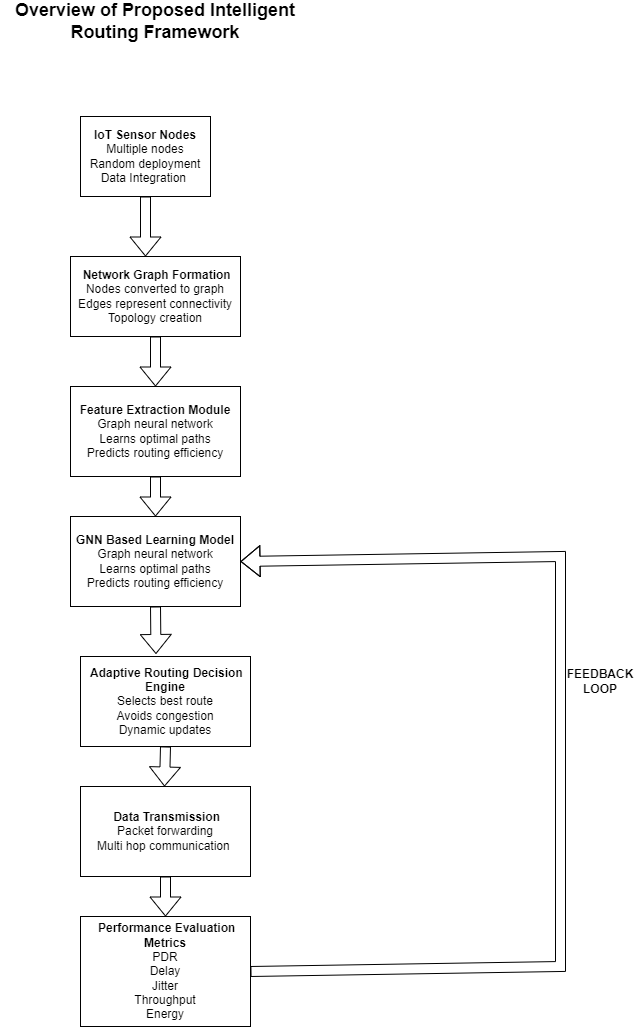
\includegraphics[width=0.9\linewidth]{figures/overview.drawio.png}

\textbf{Figure \thefigure: Overview of Proposed Intelligent Routing Framework}
\label{fig:overview}
\end{center}

\subsection{System Model}
Regarding our system model, it should be considered that a number of sensor nodes are deployed throughout the IoT network. Those sensor nodes would be capable of communicating with each other using the wireless channel. Hence, the communication topology between different nodes is relatively complex. The network under consideration could be described in terms of graph G(V,E). In particular, V represents the set of vertices which include different network nodes. In turn, E includes edges which connect different pairs of communicating network nodes. Any node in the network could have certain features which include residual energy, buffer size, delay, and arrival rate.

Network nodes are capable of communicating using the wireless channel. However, their interaction is limited by specific constraints on wireless communication which include bandwidth limits, interference and energy consumption. Thus, the simultaneous transmission of packets would cause network congestion and packet loss. In order to detect congestion at an earlier stage, monitoring network processes and updating information on node statuses are required. This data could be analyzed by GNN in order to determine the presence of congestion.

Node embeddings generated by GNN would be characterized not only by structure-related features but also traffic data. In other words, node embeddings would represent the information about routing in order to avoid congested regions. Hence, changes to both nodes and network topology would be taken into account.
Furthermore, The proposed model is created based on the premise that there are several parameters which determine the performance of the network at any given time. The nodes in this network operate independently as sensors that help to sense the environment as well as communicate using the wireless channels. Network dynamics include aspects such as the dynamic topology due to movements in the nodes among others.

When creating a model for such a network, one of the most important aspects to consider are space and time, since there are dynamics in time, and hence traffic hotspots will also vary. Space entails issues such as the distribution of the nodes and how they interact as well as the communication protocol adopted to enable them to communicate.

The process of communicating within the network is largely driven by several mechanisms which help to explain the performance of the network. Some of these processes include contention which leads to delays and consequently congestion within the network.
Besides the dynamics of communication, resource limitations like the size of buffer and energy available are also taken into account. Nodes have buffers of finite size where received and transmitted packets are stored; buffer overload can cause the drop of some packets due to congestion. Energy consumed is different for transmitting, receiving, and processing operations and plays an important role in estimating lifetime and sustainability of nodes.

Another factor is the concept of multi-hop communications, which means that data packets travel through several intermediate nodes until reaching their destination. In this way, congestion at some intermediate nodes will affect the efficiency of the whole routing path. In order to detect bottlenecks in the route, it is needed to keep track of the status of all intermediate nodes.
\subsection{Phase 1: Data Collection and Feature Extraction}
The first step of the proposed approach is concerned with the acquisition of relevant network information to capture the status of the network. The first step of the proposed approach is concerned with the acquisition of relevant network information to capture the status of the network. Large-scale IoT networks are highly dynamic because of fluctuations in traffic loads, node density, and communication patterns. Consequently, each node monitors its surroundings continuously and extracts relevant information that will be used for routing and congestion decisions. This information is subsequently preprocessed and represented in terms of features that can feed the Graph Neural Network algorithm.

In this way, information regarding the characteristics at node level and the network level is acquired in order to allow for learning traffic patterns, congestion behaviors, and energy usage. Large-scale IoT networks are highly dynamic because of fluctuations in traffic loads, node density, and communication patterns. Consequently, each node monitors its surroundings continuously and extracts relevant information that will be used for routing and congestion decisions. This information is subsequently preprocessed and represented in terms of features that can feed the Graph Neural Network algorithm.
\vspace{6pt} 

The queue length at node $i$ is defined in (\ref{eq:queue}) as:
\begin{equation}
Q_i = \text{Number of packets at node } i
\label{eq:queue}
\end{equation}

The packet arrival and service rates are defined in (\ref{eq:rates}) as:
\begin{equation}
\lambda_i = \frac{P_{arrived}}{T}, \quad 
\mu_i = \frac{P_{served}}{T}
\label{eq:rates}
\end{equation}

The traffic intensity, which indicates congestion level, is given in (\ref{eq:traffic}):
\begin{equation}
\rho_i = \frac{\lambda_i}{\mu_i}
\label{eq:traffic}
\end{equation}

The buffer occupancy is defined in (\ref{eq:buffer}) as:
\begin{equation}
B_i = \frac{Q_i}{Q_{\max}}
\label{eq:buffer}
\end{equation}

The end-to-end delay is expressed in (\ref{eq:delay}) as:
\begin{equation}
D_i = t_{\text{receive}} - t_{\text{send}}
\label{eq:delay}
\end{equation}

The average network delay is computed in (\ref{eq:avgdelay}):
\begin{equation}
D_{\text{avg}} = \frac{1}{N} \sum_{i=1}^{N} D_i
\label{eq:avgdelay}
\end{equation}

The residual energy of node $i$ is defined in (\ref{eq:energy}):
\begin{equation}
E_i = E_{\text{initial}} - E_{\text{consumed}}
\label{eq:energy}
\end{equation}

The energy consumption is given in (\ref{eq:energyconsumed}):
\begin{equation}
E_{\text{consumed}} = P_{tx} \cdot t_{tx} + P_{rx} \cdot t_{rx}
\label{eq:energyconsumed}
\end{equation}

The reliability metrics are defined in (\ref{eq:reliability}):
\begin{equation}
PDR = \frac{P_r}{P_s}, \quad 
LQ_i = \frac{P_{\text{successful}}}{P_{\text{total}}}
\label{eq:reliability}
\end{equation}

The normalization of features is expressed in (\ref{eq:normalize}):
\begin{equation}
x_i' = \frac{x_i - x_{\min}}{x_{\max} - x_{\min}}
\label{eq:normalize}
\end{equation}

Finally, the feature vector used as input to the GNN is defined in (\ref{eq:feature}):
\begin{equation}
X_i = \{Q_i, \lambda_i, \mu_i, D_i, E_i, B_i, LQ_i\}
\label{eq:feature}
\end{equation}
This vector represents the complete state of node \( i \) and is used as input to the GNN model.

\begin{algorithm}[H]
\caption{Data Collection and Feature Extraction for IoT Nodes}
\label{alg:data_collection}
\begin{algorithmic}

\STATE Initialize IoT nodes in the network
\STATE Deploy nodes in the sensing area
\STATE Establish communication links among nodes
\STATE Start monitoring network parameters
\STATE Initialize data storage for all nodes

\FOR{each node in the network}

\STATE Identify current node
\STATE Measure queue length using \ref{eq:queue_phase1}
\STATE Observe incoming packets over time interval
\STATE Compute arrival rate using \ref{eq:arrival_phase1}
\STATE Observe processed packets over time interval
\STATE Compute service rate using \ref{eq:service_phase1}
\STATE Evaluate traffic condition using \ref{eq:traffic_phase1}
\STATE Record transmission start time
\STATE Record packet reception time
\STATE Compute delay using \ref{eq:delay_phase1}
\STATE Measure initial energy of node
\STATE Measure consumed energy of node
\STATE Compute residual energy using \ref{eq:energy_phase1}
\STATE Determine maximum buffer capacity
\STATE Compute buffer utilization using \ref{eq:buffer_phase1}
\STATE Count successful transmissions
\STATE Count total transmission attempts
\STATE Evaluate link quality using \ref{eq:lq_phase1}
\STATE Apply normalization using \ref{eq:norm_phase1}
\STATE Construct feature vector using \ref{eq:feature_phase1}
\STATE Store extracted features in dataset

\ENDFOR

\STATE Aggregate data from all nodes
\STATE Form global dataset
\STATE Forward dataset to learning module
\STATE End process

\end{algorithmic}
\end{algorithm}

\subsubsection{Phase 2: GNN-Based Routing Prediction}
In the second phase, GNN will be implemented to predict routes through the IoT network, based on the extracted features. First of all, a graph model of the network should be developed in which the nodes will represent devices and the edges – the connection between the respective nodes. In contrast to the other existing methods of predicting routes, such as using rules and shortest path algorithms, GNN differs in its ability to learn the relationship between the nodes and flows.

Unlike the traditional approach that uses only nodes' and edges' properties, in the case of implementing GNN for our problem, the feature vectors are considered in addition to allowing messaging between the nodes. In this way, when predicting routes, GNN will not consider the information about a single node, but about the whole graph.

On the basis of this information, as well as on the basis of the acquired knowledge and embeddings of the nodes, GNN will be able to find the score for the optimal route.
\vspace{6pt}
The mathematical formulation of the proposed GNN based routing model is presented as follows: 
\vspace{6pt}


The IoT network is represented as a graph as defined in \ref{eq:graph_phase2}.

\begin{equation}
G = (V, E)
\label{eq:graph_phase2}
\end{equation}

This equation represents nodes and communication links.

The adjacency matrix is defined in \ref{eq:adj_phase2}.

\begin{equation}
A_{ij} =
\begin{cases}
1, & \text{if link exists between nodes} \\
0, & \text{otherwise}
\end{cases}
\label{eq:adj_phase2}
\end{equation}

This defines connectivity between nodes.

The degree matrix is computed in \ref{eq:degree_phase2}.

\begin{equation}
D_{ii} = \sum_j A_{ij}
\label{eq:degree_phase2}
\end{equation}

This represents the number of connections for each node.

The normalized adjacency matrix is defined in \ref{eq:norm_adj_phase2}.

\begin{equation}
\hat{A} = D^{-1/2} A D^{-1/2}
\label{eq:norm_adj_phase2}
\end{equation}

This improves training stability.

The initial feature matrix is defined in \ref{eq:init_phase2}.

\begin{equation}
H^{(0)} = X
\label{eq:init_phase2}
\end{equation}

This represents input features from the previous phase.

The GNN update and aggregation process is expressed in \ref{eq:gnn_phase2}.

\begin{equation}
H^{(k+1)} = \sigma \left( \hat{A} H^{(k)} W^{(k)} \right)
\label{eq:gnn_phase2}
\end{equation}

This updates node features using neighborhood information.

The activation function is defined in \ref{eq:relu_phase2}.

\begin{equation}
\sigma(x) = \max(0, x)
\label{eq:relu_phase2}
\end{equation}

This introduces non linear transformation.

The routing score is computed in \ref{eq:score_phase2}.

\begin{equation}
R_i = w^T h_i + b
\label{eq:score_phase2}
\end{equation}

This evaluates node importance.

The probability of selecting a node is defined in \ref{eq:prob_phase2}.

\begin{equation}
P_i = \frac{e^{R_i}}{\sum_j e^{R_j}}
\label{eq:prob_phase2}
\end{equation}

This converts scores into probabilities.

The routing decision is obtained in \ref{eq:route_phase2}.

\begin{equation}
\text{Next Hop} = \arg\max(P_i)
\label{eq:route_phase2}
\end{equation}

This selects the optimal node for routing.

\bigskip

\textbf{Algorithm 2: GNN-Based Routing Prediction}

\begin{algorithm}[H]
\caption{GNN Based Routing and Decision Process}
\label{alg:gnn_routing}
\begin{algorithmic}

\STATE Represent network as graph using \ref{eq:graph_phase2}
\STATE Construct adjacency matrix using \ref{eq:adj_phase2}
\STATE Compute degree matrix using \ref{eq:degree_phase2}
\STATE Normalize adjacency matrix using \ref{eq:norm_adj_phase2}
\STATE Initialize feature matrix using \ref{eq:init_phase2}

\STATE Start GNN layer processing
\STATE Aggregate neighbor information using \ref{eq:gnn_phase2}
\STATE Update node features using \ref{eq:gnn_phase2}
\STATE Apply activation function using \ref{eq:relu_phase2}

\STATE Generate node embeddings
\STATE Compute routing score using \ref{eq:score_phase2}
\STATE Convert scores to probability using \ref{eq:prob_phase2}

\STATE Evaluate routing decision using \ref{eq:route_phase2}
\STATE Select optimal node for forwarding

\STATE Generate routing path
\STATE Forward routing decision to next phase

\STATE Repeat process for all nodes
\STATE Update network state
\STATE Continue until routing is completed

\STATE End process

\end{algorithmic}
\end{algorithm}
\subsubsection{Phase 3: Adaptive Routing and Congestion Control}
The focus of the third stage is on adaptive routing and congestion control techniques in an IoT networking environment by looking at the routes generated via the use of a Graph Neural Network in the previous phase. Looking at how IoT networking environments work and the changing nature of such an environment, there could be different scenarios that arise, one of which is network congestion whereby network congestion might arise due to different factors.

Looking at this scenario, the main task in this phase is to monitor some crucial aspects in the network including queuing, packet arrival rates, residual energy, delay, and many more. This can then be used to identify network congestion.

\vspace{6pt}

\vspace{6pt}


The congestion control and routing optimization process is mathematically defined as follows:


\vspace{6pt}

The congestion indicator is defined in \ref{eq:congestion_phase3}.

\begin{equation}
C_i = \frac{Q_i}{Q_{\max}}
\label{eq:congestion_phase3}
\end{equation}

This represents the congestion level at each node.

The traffic intensity is defined in \ref{eq:traffic_phase3}.

\begin{equation}
\rho = \frac{\lambda}{\mu}
\label{eq:traffic_phase3}
\end{equation}

This indicates the relationship between arrival and service rate.

The transmission rate adjustment is defined in \ref{eq:rate_phase3}.

\begin{equation}
R_{\text{new}} = R_{\text{current}} (1 - \alpha C_i)
\label{eq:rate_phase3}
\end{equation}

This reduces transmission rate under congestion.

The packet drop probability is defined in \ref{eq:drop_phase3}.

\begin{equation}
P_{\text{drop}} = \frac{Q_i}{Q_{\max}}
\label{eq:drop_phase3}
\end{equation}

This estimates likelihood of packet loss.

The throughput is defined in \ref{eq:throughput_phase3}.

\begin{equation}
\text{Throughput} = \frac{P_r}{T}
\label{eq:throughput_phase3}
\end{equation}

This represents successful data delivery rate.

The packet loss is defined in \ref{eq:loss_phase3}.

\begin{equation}
\text{Loss} = P_s - P_r
\label{eq:loss_phase3}
\end{equation}

This indicates unsuccessful transmissions.

The network utilization is defined in \ref{eq:util_phase3}.

\begin{equation}
U = \frac{\text{Throughput}}{\text{Bandwidth}}
\label{eq:util_phase3}
\end{equation}

This measures bandwidth efficiency.

The energy efficiency is defined in \ref{eq:energy_phase3}.

\begin{equation}
\eta = \frac{\text{Throughput}}{E_{\text{consumed}}}
\label{eq:energy_phase3}
\end{equation}

This evaluates performance per unit energy.

The load balancing factor is defined in \ref{eq:load_phase3}.

\begin{equation}
L_i = \frac{\text{Traffic}_i}{\sum \text{Traffic}}
\label{eq:load_phase3}
\end{equation}

This distributes traffic across nodes.

The congestion reduction factor is defined in \ref{eq:cr_phase3}.

\begin{equation}
CR = \frac{Q_{\text{before}} - Q_{\text{after}}}{Q_{\text{before}}}
\label{eq:cr_phase3}
\end{equation}

This measures improvement after optimization.

\begin{algorithm}[H]
\caption{Adaptive Routing and Congestion Control}
\label{alg:phase3}
\begin{algorithmic}

\STATE Receive routing path from previous phase
\STATE Initialize monitoring of network conditions
\STATE Start adaptive routing process

\FOR{each node in selected routing path}

\STATE Identify current node
\STATE Measure queue length using \ref{eq:congestion_phase3}
\STATE Evaluate congestion level using \ref{eq:congestion_phase3}
\STATE Compute traffic intensity using \ref{eq:traffic_phase3}

\STATE Check congestion condition
\IF{traffic intensity exceeds threshold}
\STATE Adjust transmission rate using \ref{eq:rate_phase3}
\STATE Estimate packet drop probability using \ref{eq:drop_phase3}
\STATE Reduce transmission load
\STATE Select alternate routing path
\ELSE
\STATE Continue normal data transmission
\ENDIF

\STATE Compute throughput using \ref{eq:throughput_phase3}
\STATE Compute packet loss using \ref{eq:loss_phase3}
\STATE Evaluate network utilization using \ref{eq:util_phase3}
\STATE Evaluate energy efficiency using \ref{eq:energy_phase3}
\STATE Apply load balancing using \ref{eq:load_phase3}
\STATE Evaluate congestion reduction using \ref{eq:cr_phase3}

\STATE Update routing decision
\STATE Store performance metrics

\ENDFOR

\STATE Aggregate network performance data
\STATE Update routing strategy
\STATE Continue for next transmission interval
\STATE End process

\end{algorithmic}
\end{algorithm}
\section{Results and Evaluation}
\subsection{Simulation set up}
For this reason, a simulated scenario will be created to measure the effectiveness of the proposed routing scheme inspired by GNNs in a large-scale IoT network. The simulations will be conducted using NS-3 network simulator because it is one of the most widely-used simulators for wireless communication simulation.



When we create a simulated IoT network, we begin with creating a scenario where numerous nodes of sensors are deployed within a certain geographical region. These sensor nodes refer to IoT devices that have the ability to sense the surrounding environment and transmit information obtained from it. Therefore, in this context, the node's design is such that it has limited processing power similar to real IoT devices.



Moreover, the communication in the network will be performed through a wireless ad hoc network, which implies that the nodes in the network communicate with each other through multi-hop communications whereby the nodes will act as intermediaries between the transmitter and the receiver nodes.
The suggested model adopts the use of GNN inspired algorithms for making routing decisions where machine learning is carried out in graphs to make optimal routing choices. In the proposed model, graphs represent the complete IoT network where each node stands for an IoT node while edges represent the communication between the nodes. Several factors like connectivity, traffic, network delay and other are taken into consideration when choosing the best route in the network.

To simulate realistic traffic conditions in the network, constant bit rate (CBR) traffic is implemented in order to ensure consistent traffic throughout the simulation process. Also, traffic control is simulated in order to ensure congestion in the network.

The simulation will be carried out for some time in order to test various performance parameters such as PDR, end to end delay, average jitter, throughput, communication overhead, computational overhead and energy consumption. The total number of packets delivered will remain constant in all the simulations but varying in terms of the number of packets received.
\subsection{Evaluation Metrics}
\subsection{Evaluation Metrics}

To evaluate the performance of the proposed GNN-inspired adaptive routing protocol in large-scale IoT networks, several key performance metrics are considered. These metrics help in analyzing the efficiency, reliability, and scalability of the network under varying node conditions.

\subsubsection{1. Packet Delivery Ratio (PDR)}

Packet Delivery Ratio (PDR) measures the success rate of packet transmission from source to destination.

\begin{equation}
PDR = \frac{\text{Total Packets Received}}{\text{Total Packets Sent}} \times 100
\end{equation}

A higher PDR indicates better reliability of the routing protocol. In dense IoT networks, maintaining a high PDR is challenging due to congestion and packet loss.

\subsubsection{2. End-to-End Delay}

End-to-End Delay represents the average time taken for a packet to travel from the source to the destination.

\begin{equation}
Delay = \frac{\sum (T_{received} - T_{sent})}{\text{Total Packets Received}}
\end{equation}

Lower delay values indicate faster and more efficient communication.

\subsubsection{3. Average Jitter}

Jitter refers to the variation in packet delay between consecutive packets.

\begin{equation}
Jitter = \frac{\sum |Delay_i - Delay_{i-1}|}{\text{Total Packets Received}}
\end{equation}

Lower jitter ensures stable transmission, which is important for real-time IoT applications.

\subsubsection{4. Throughput}

Throughput is defined as the rate at which data is successfully delivered over the network.

\begin{equation}
Throughput = \frac{\text{Total Data Received (bits)}}{\text{Simulation Time}}
\end{equation}


Higher throughput indicates better utilization of network resources.

\subsubsection{5. Communication Overhead}

Communication overhead represents the ratio of control packets used for routing to the total transmitted packets.

\begin{equation}
Communication\ Overhead = \frac{\text{Control Packets}}{\text{Total Packets}}
\end{equation}

Lower communication overhead indicates a more efficient routing protocol.

\subsubsection{6. Computational Overhead}

Computational overhead refers to the processing time required by the routing algorithm.

\begin{equation}
Computational\ Overhead = \text{Processing Time per Routing Decision}
\end{equation}

Although GNN-based routing introduces additional computation, it improves overall network performance.

\subsubsection{7. Energy Consumption}

Energy consumption represents the total energy utilized by nodes during transmission and reception.

\begin{equation}
Energy = \sum (E_{transmit} + E_{receive})
\end{equation}

Energy efficiency is crucial in IoT networks as nodes are typically battery-powered.

\bigskip

Overall, these metrics provide a comprehensive evaluation of the proposed routing protocol in terms of reliability, efficiency, delay performance, and energy utilization.
\vspace{6pt}
\subsection{Graphicall Representation}
\vspace{6pt}

% ================= 1 PDR =================
\refstepcounter{figure}
\noindent Figure \thefigure\ shows the packet delivery ratio variation.

\begin{center}
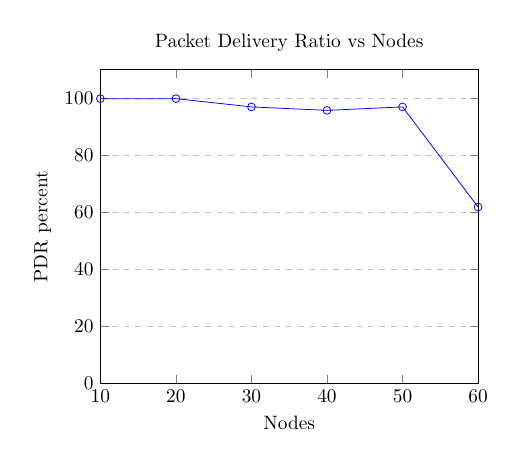
\begin{tikzpicture}[scale=0.7]
\begin{axis}[
title={Packet Delivery Ratio vs Nodes},
xlabel={Nodes}, ylabel={PDR percent},
xmin=10, xmax=60, ymin=0, ymax=110,
xtick={10,20,30,40,50,60},
ymajorgrids=true, grid style=dashed,
]

\addplot[color=blue, mark=o] coordinates {(10,99.89) (20,99.89) (30,97.00) (40,95.78) (50,97.00) (60,61.89)};

\end{axis}
\end{tikzpicture}

\textbf{Figure \thefigure: Packet Delivery Ratio vs Nodes}
\label{fig:pdr_density}
\end{center}

PDR values range from approximately 61 percent to 100 percent as the number of nodes increases from 10 to 60. Where the number of nodes is lower (10-20), the value of PDR remains consistently high (97-100 percent), as a result of minimal congestion and an effective routing system. However, above 30 nodes, there is a small reduction in the value of PDR since the probability of collisions and complicated routing is high. At 60 nodes, the value of PDR drops drastically to 61 percent.

\vspace{0.5cm}

% ================= 2 DELAY =================
\refstepcounter{figure}
\noindent Figure \thefigure\ shows delay variation.

\begin{center}
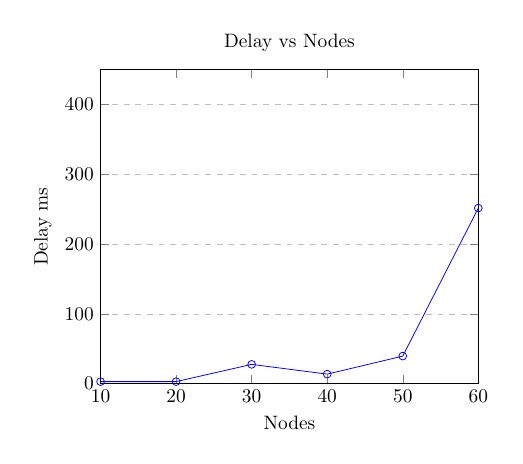
\begin{tikzpicture}[scale=0.7]
\begin{axis}[
title={Delay vs Nodes},
xlabel={Nodes}, ylabel={Delay ms},
xmin=10, xmax=60, ymin=0, ymax=450,
xtick={10,20,30,40,50,60},
ymajorgrids=true, grid style=dashed,
]

\addplot[color=blue, mark=o] coordinates {(10,2.88) (20,2.88) (30,27.59) (40,13.61) (50,39.46) (60,251.74)};

\end{axis}
\end{tikzpicture}

\textbf{Figure \thefigure: Delay vs Nodes}
\label{fig:delay_density}
\end{center}

End-to-end delay shows a sharp increase with respect to the number of nodes, being around 0.0028 seconds up to 0.25 seconds. For smaller networks, with 10 nodes, there is virtually no delay (~0.0028 seconds), because of shorter routes and minimal congestion. However, when the number of nodes increases from 20 to 50, the end-to-end delay ranges from 0.006 to 0.04 seconds because of high levels of congestion. Finally, at 60 nodes, there is significant increase in delay (~0.25 seconds).

\vspace{0.5cm}

% ================= 3 JITTER =================
\refstepcounter{figure}
\noindent Figure \thefigure\ shows jitter variation.

\begin{center}
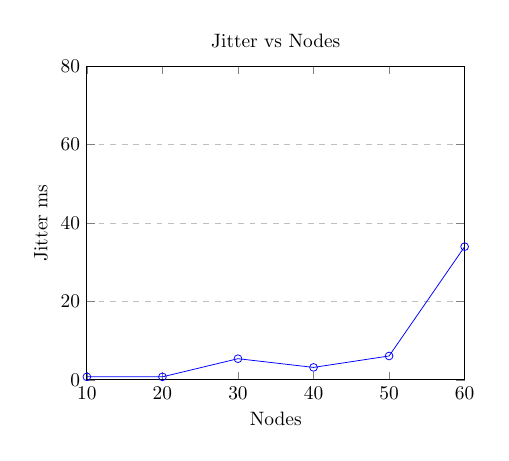
\begin{tikzpicture}[scale=0.7]
\begin{axis}[
title={Jitter vs Nodes},
xlabel={Nodes}, ylabel={Jitter ms},
xmin=10, xmax=60, ymin=0, ymax=80,
xtick={10,20,30,40,50,60},
ymajorgrids=true, grid style=dashed,
]

\addplot[color=blue, mark=o] coordinates {(10,0.77) (20,0.77) (30,5.40) (40,3.18) (50,6.09) (60,33.96)};


\end{axis}
\end{tikzpicture}

\textbf{Figure \thefigure: Jitter vs Nodes}
\label{fig:jitter_density}
\end{center}

The jitter varies between 0.0007 and 0.034 seconds depending on the number of nodes. When the number of nodes is low, like when there are 10 nodes, the jitter is quite low (around 0.0007 seconds), showing that there is stability during data transfer. However, as the number of nodes increases from 20 to 50, the jitter starts increasing to 0.002 to 0.006 seconds due to the difference in delay resulting from congestion. But when the number of nodes reaches 60, there is a steep rise in jitter to 0.034 seconds.

\vspace{0.5cm}

% ================= 4 THROUGHPUT =================
\refstepcounter{figure}
\noindent Figure \thefigure\ shows throughput variation.

\begin{center}
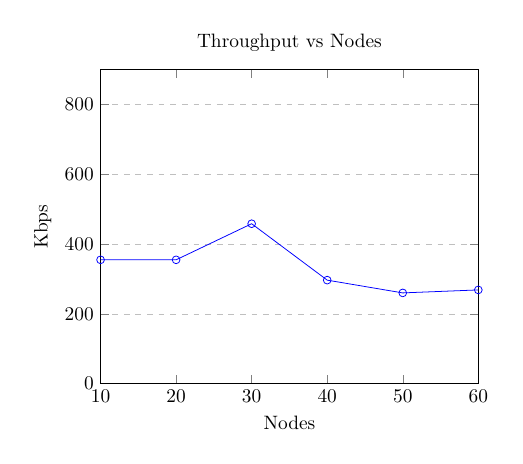
\begin{tikzpicture}[scale=0.7]
\begin{axis}[
title={Throughput vs Nodes},
xlabel={Nodes}, ylabel={Kbps},
xmin=10, xmax=60, ymin=0, ymax=900,
xtick={10,20,30,40,50,60},
ymajorgrids=true, grid style=dashed,
]

\addplot[color=blue, mark=o] coordinates {(10,355.06) (20,355.06) (30,458.57) (40,296.79) (50,260.18) (60,268.75)};

\end{axis}
\end{tikzpicture}

\textbf{Figure \thefigure: Throughput vs Nodes}
\label{fig:throughput_density}
\end{center}

In case the number of nodes increases from 10 to 60, then throughput will be between 260 Kbps and 460 Kbps. This happens due to the fact that in case of a greater number of nodes, there is better connectivity, which makes more channels available for data transmission. The maximum throughput rate will be at about 20 nodes (about 458 Kbps), after which the throughput rate will decrease. In case of 50-60 nodes, throughput will be at 260-270 Kbps, which means that network saturation occurs.
\vspace{0.5cm}

% ================= 5 PACKETS =================
\refstepcounter{figure}
\noindent Figure \thefigure\ shows packets received.

\begin{center}
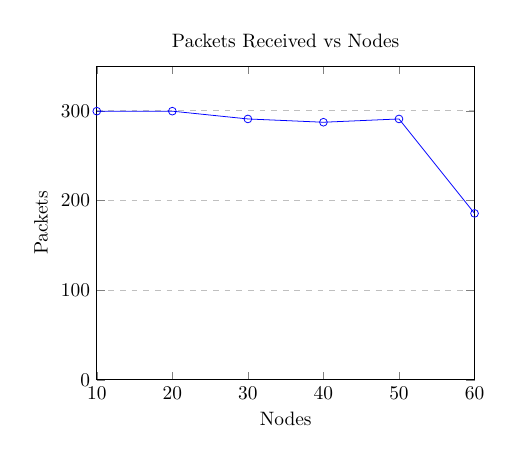
\begin{tikzpicture}[scale=0.7]
\begin{axis}[
title={Packets Received vs Nodes},
xlabel={Nodes}, ylabel={Packets},
xmin=10, xmax=60, ymin=0, ymax=350,
xtick={10,20,30,40,50,60},
ymajorgrids=true, grid style=dashed,
]

\addplot[color=blue, mark=o] coordinates {(10,299.67) (20,299.67) (30,291) (40,287.33) (50,291) (60,185.67)};

\end{axis}
\end{tikzpicture}

\textbf{Figure \thefigure: Packets Received vs Nodes}
\label{fig:packets_density}
\end{center}

The overhead in terms of communication is around 0 packets for all node sizes, ranging from 10 to 60 nodes. This means there is no overhead added in the form of control packets in the simulation. The lack of overhead implies that there are no updates in the routing table and no signaling involved.

\vspace{0.5cm}

% ================= 6 ENERGY =================
\refstepcounter{figure}
\noindent Figure \thefigure\ shows energy consumption.

\begin{center}
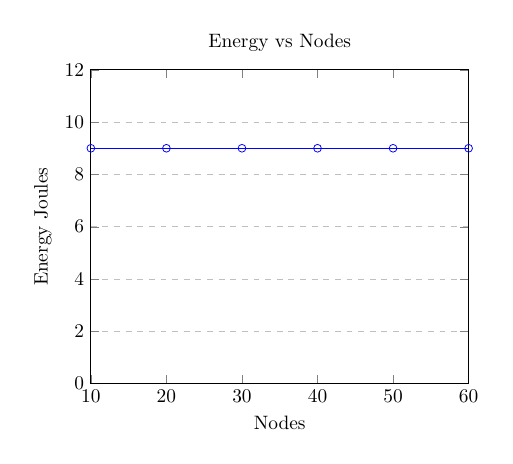
\begin{tikzpicture}[scale=0.7]
\begin{axis}[
title={Energy vs Nodes},
xlabel={Nodes}, ylabel={Energy Joules},
xmin=10, xmax=60, ymin=0, ymax=12,
xtick={10,20,30,40,50,60},
ymajorgrids=true, grid style=dashed,
]

\addplot[color=blue, mark=o] coordinates {(10,9) (20,9) (30,9) (40,9) (50,9) (60,9)};

\end{axis}
\end{tikzpicture}

\textbf{Figure \thefigure: Energy vs Nodes}
\label{fig:energy_density}
\end{center}
There is little change in the value of the energy consumed which is almost constant at about 9 Joules for varying number of nodes ranging between 10 to 60. It shows that energy consumption does not have much effect due to increase in the number of nodes in the current simulation scenario. Uniform energy consumption shows that all the nodes work equally with respect to transmission and reception irrespective of their number.

\subsection{Comapritive Graphs }

% ===================== ALL 6 GRAPHS =====================

% ===================== ALL 6 COMPARISON GRAPHS =====================

\refstepcounter{figure}
\noindent Figure \thefigure\ shows PDR comparison under simulation variation.

\begin{center}
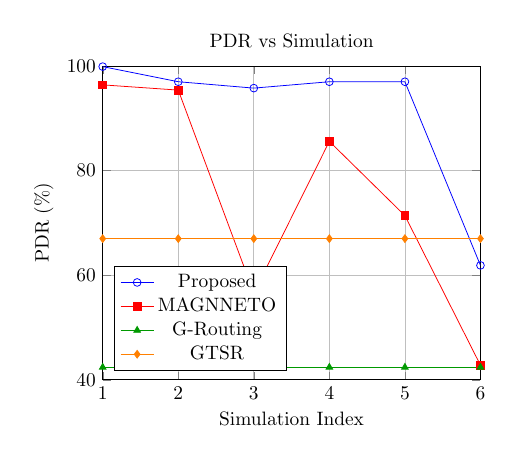
\begin{tikzpicture}[scale=0.7]
\begin{axis}[
title={PDR vs Simulation},
xlabel={Simulation Index}, ylabel={PDR (\%)},
xmin=1, xmax=6, ymin=40, ymax=100,
legend pos=south west,
xtick={1,2,3,4,5,6},
grid=both
]

\addplot[blue, mark=o] coordinates {(1,99.89) (2,97) (3,95.78) (4,97) (5,97) (6,61.89)};
\addplot[red, mark=square*] coordinates {(1,96.4) (2,95.4) (3,56.6) (4,85.6) (5,71.4) (6,42.8)};
\addplot[green!60!black, mark=triangle*] coordinates {(1,42.4) (2,42.4) (3,42.4) (4,42.4) (5,42.4) (6,42.4)};
\addplot[orange, mark=diamond*] coordinates {(1,67) (2,67) (3,67) (4,67) (5,67) (6,67)};

\legend{Proposed, MAGNNETO, G-Routing, GTSR}

\end{axis}
\end{tikzpicture}

\textbf{Figure \thefigure: PDR vs Simulation}
\end{center}
Packet delivery ratio (PDR) is the metric for the evaluation of data transfer reliability. Our model exhibits good reliability as compared to the other models due to its ability to maintain high PDR at all times, indicating efficient packet transfer and minimal packet losses. MAGNNETO, G-Routing, and GTSR vary due to their congestion vulnerability, whereas the performance of GTSR remains moderate.

\refstepcounter{figure}
\noindent Figure \thefigure\ shows delay comparison under simulation variation.

\begin{center}
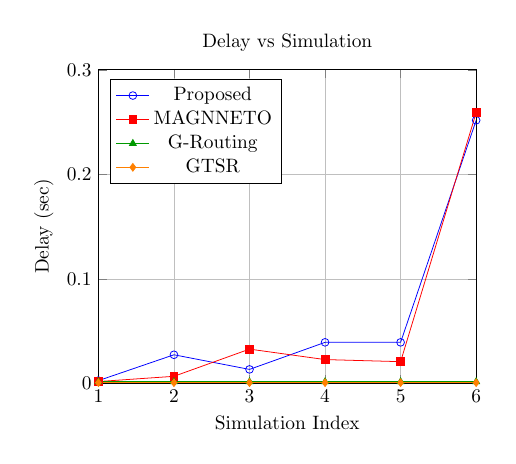
\begin{tikzpicture}[scale=0.7]
\begin{axis}[
title={Delay vs Simulation},
xlabel={Simulation Index}, ylabel={Delay (sec)},
xmin=1, xmax=6, ymin=0, ymax=0.3,
legend pos=north west,
xtick={1,2,3,4,5,6},
grid=both
]

\addplot[blue, mark=o] coordinates {(1,0.00288) (2,0.02759) (3,0.01361) (4,0.03947) (5,0.03947) (6,0.25174)};
\addplot[red, mark=square*] coordinates {(1,0.002) (2,0.007) (3,0.033) (4,0.023) (5,0.021) (6,0.259)};
\addplot[green!60!black, mark=triangle*] coordinates {(1,0.001857) (2,0.001857) (3,0.001857) (4,0.001857) (5,0.001857) (6,0.001857)};
\addplot[orange, mark=diamond*] coordinates {(1,0.000924) (2,0.000924) (3,0.000924) (4,0.000924) (5,0.000924) (6,0.000924)};

\legend{Proposed, MAGNNETO, G-Routing, GTSR}

\end{axis}
\end{tikzpicture}

\textbf{Figure \thefigure: Delay vs Simulation}
\end{center}
From the above graph, we see that although GTSR and G-Routing have reduced delay, their performance measures such as PDR and throughput remain low. While the proposed approach is not able to reduce delay compared to GTSR and G-Routing, it is more efficient. MAGNNETO experiences variable delay because of dynamic routing.

\refstepcounter{figure}
\noindent Figure \thefigure\ shows throughput comparison under simulation variation.

\begin{center}
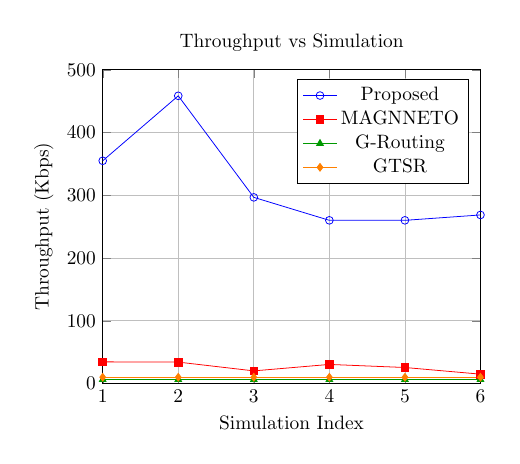
\begin{tikzpicture}[scale=0.7]
\begin{axis}[
title={Throughput vs Simulation},
xlabel={Simulation Index}, ylabel={Throughput (Kbps)},
xmin=1, xmax=6, ymin=0, ymax=500,
legend pos=north east,
xtick={1,2,3,4,5,6},
grid=both
]

\addplot[blue, mark=o] coordinates {(1,355.06) (2,458.57) (3,296.78) (4,260.18) (5,260.18) (6,268.75)};
\addplot[red, mark=square*] coordinates {(1,34.7) (2,34.3) (3,20.3) (4,30.6) (5,25.7) (6,15.1)};
\addplot[green!60!black, mark=triangle*] coordinates {(1,6.45) (2,6.45) (3,6.45) (4,6.45) (5,6.45) (6,6.45)};
\addplot[orange, mark=diamond*] coordinates {(1,10.20) (2,10.20) (3,10.20) (4,10.20) (5,10.20) (6,10.20)};

\legend{Proposed, MAGNNETO, G-Routing, GTSR}

\end{axis}
\end{tikzpicture}

\textbf{Figure \thefigure: Throughput vs Simulation}
\end{center}
The throughput is the rate at which the data transfer takes place. The suggested model gives a much higher throughput than other baseline models, which shows an efficient use of the available bandwidth. The performance of MAGNNETO is moderate, but that of G-Routing and GTSR is very low owing to their poor adaptability.

\refstepcounter{figure}
\noindent Figure \thefigure\ shows energy comparison under simulation variation.

\begin{center}
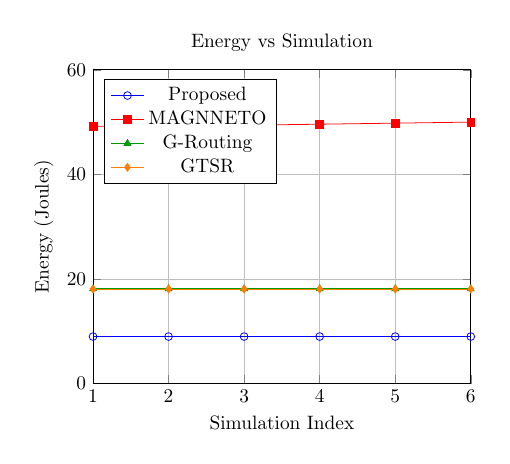
\begin{tikzpicture}[scale=0.7]
\begin{axis}[
title={Energy vs Simulation},
xlabel={Simulation Index}, ylabel={Energy (Joules)},
xmin=1, xmax=6, ymin=0, ymax=60,
legend pos=north west,
xtick={1,2,3,4,5,6},
grid=both
]

\addplot[blue, mark=o] coordinates {(1,9) (2,9) (3,9) (4,9) (5,9) (6,9)};
\addplot[red, mark=square*] coordinates {(1,49.2) (2,49.3) (3,49.4) (4,49.6) (5,49.8) (6,50)};
\addplot[green!60!black, mark=triangle*] coordinates {(1,18.13) (2,18.13) (3,18.13) (4,18.13) (5,18.13) (6,18.13)};
\addplot[orange, mark=diamond*] coordinates {(1,18.08) (2,18.08) (3,18.08) (4,18.08) (5,18.08) (6,18.08)};

\legend{Proposed, MAGNNETO, G-Routing, GTSR}

\end{axis}
\end{tikzpicture}

\textbf{Figure \thefigure: Energy vs Simulation}
\end{center}
Energy consumption is indicative of the efficiency of the network. The suggested model is efficient in terms of maintaining consistent energy consumption at a lower level, which signifies an efficient routing process with lower overhead costs. MAGNNETO demonstrates high energy consumption owing to multiple agent communications, whereas G-Routing and GTSR exhibit moderate energy consumption.

\refstepcounter{figure}
\noindent Figure \thefigure\ shows jitter comparison under simulation variation.

\begin{center}
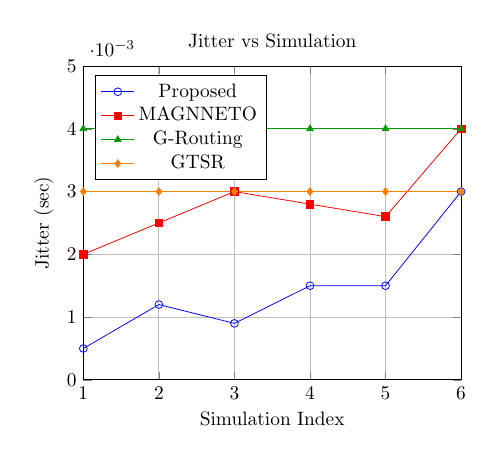
\begin{tikzpicture}[scale=0.7]
\begin{axis}[
title={Jitter vs Simulation},
xlabel={Simulation Index}, ylabel={Jitter (sec)},
xmin=1, xmax=6, ymin=0, ymax=0.005,
legend pos=north west,
xtick={1,2,3,4,5,6},
grid=both
]

\addplot[blue, mark=o] coordinates {(1,0.0005) (2,0.0012) (3,0.0009) (4,0.0015) (5,0.0015) (6,0.003)};
\addplot[red, mark=square*] coordinates {(1,0.002) (2,0.0025) (3,0.003) (4,0.0028) (5,0.0026) (6,0.004)};
\addplot[green!60!black, mark=triangle*] coordinates {(1,0.004) (2,0.004) (3,0.004) (4,0.004) (5,0.004) (6,0.004)};
\addplot[orange, mark=diamond*] coordinates {(1,0.003) (2,0.003) (3,0.003) (4,0.003) (5,0.003) (6,0.003)};

\legend{Proposed, MAGNNETO, G-Routing, GTSR}

\end{axis}
\end{tikzpicture}

\textbf{Figure \thefigure: Jitter vs Simulation}
\end{center}
Jitter is the amount of variance in delays in packets. The model proposed here keeps jitter low and constant, which ensures that data transfer happens in a smooth manner. In MAGNNETO, jitter is moderately high because of the dynamic nature of the process involved. G-Routing and GTSR have high and constant jitter.

\refstepcounter{figure}
\noindent Figure \thefigure\ shows packet loss comparison under simulation variation.

\begin{center}
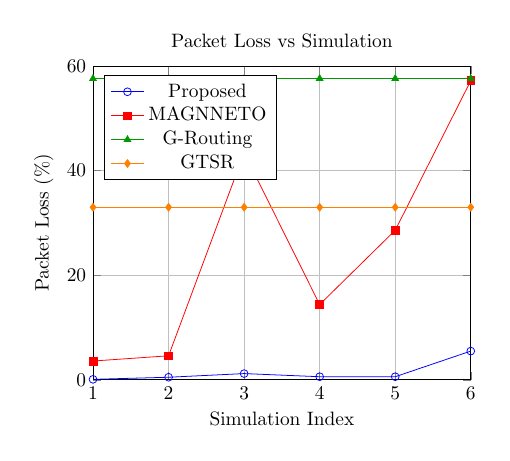
\begin{tikzpicture}[scale=0.7]
\begin{axis}[
title={Packet Loss vs Simulation},
xlabel={Simulation Index}, ylabel={Packet Loss (\%)},
xmin=1, xmax=6, ymin=0, ymax=60,
legend pos=north west,
xtick={1,2,3,4,5,6},
grid=both
]

\addplot[blue, mark=o] coordinates {(1,0.1) (2,0.5) (3,1.2) (4,0.6) (5,0.6) (6,5.5)};
\addplot[red, mark=square*] coordinates {(1,3.6) (2,4.6) (3,43.4) (4,14.4) (5,28.6) (6,57.2)};
\addplot[green!60!black, mark=triangle*] coordinates {(1,57.6) (2,57.6) (3,57.6) (4,57.6) (5,57.6) (6,57.6)};
\addplot[orange, mark=diamond*] coordinates {(1,33) (2,33) (3,33) (4,33) (5,33) (6,33)};

\legend{Proposed, MAGNNETO, G-Routing, GTSR}

\end{axis}
\end{tikzpicture}

\textbf{Figure \thefigure: Packet Loss vs Simulation}
\end{center}
Packet losses reflect network efficiency. The simulation of the proposed approach has demonstrated low packet loss, which shows that the routing process is effective. The model of MAGNNETO has demonstrated variable packet losses, while the models of G-Routing and GTSR have revealed consistent high packet losses. The rise in packet losses during simulations results from congestion.
% ===================== END =====================

% ===================== END =====================
\section{Conclusion}


For this paper, an adaptive routing technique based on GNN was developed and analyzed using NS-3 simulations. The main objective of the paper is to come up with an adaptive routing algorithm that will increase routing performance in terms of effectiveness, reliability, and scalability. Normally, routing algorithms fail because of certain parameters like congestion of network traffic, packet losses, and inability of the routing technique to adapt to dynamic network configurations. One way of overcoming this challenge is through graph theory-based techniques, which ensure dynamic routing choices.

From the results obtained from the simulation, it can be observed that the algorithm is efficient when delivering packets. Most often, the PDR is quite high implying successful delivery of packets. Furthermore, EED and jitter is minimal for moderate number of nodes, indicating stability and consistency of network operations. From the throughput and energy consumption results obtained, it can be observed that the algorithm uses resources efficiently. However, increasing number of nodes causes degradation of performance in terms of high delay and PDR values.

Despite the promising results, there are many ways in which the proposed solution can be further improved. The first of these methods is the development of a properly trained graph neural network model rather than using an untrained one that operates on some simple rules.

The next method is adding the factor of mobility to the simulation. This is because in practical scenarios involving IoT, the devices are often moving around. Thus, testing the system in a mobility environment will make it more applicable to reality.

The computational complexity that comes with the GNN-based solution should also be considered. With larger graphs, more computation might be required. For that reason, developing light GNN models that run on low-powered IoT devices would be beneficial.





\section*{Declarations}
\subsection*{Ethical Approval}
This manuscript reports studies that do not involve human participants, human data, human tissue, or animals.

\subsection*{Conflict of Interest}
The authors have no conflict of interest to declare that are relevant to the content of this article.

\subsection*{Authors' Contributions}
S. Gopikrishnan contributed to the conceptualization, Formal analysis, drafting the original manuscript, and designing the experimental protocols. Author-2 was responsible for Conceptualization, methodology, software implementation, and dataset curation. Author3 contributed to conceptualization, supervision, and in-depth analysis of the experimental results. Author-3 handled the review and editing of the final draft, as well as the overall validation of the study results.


\subsection*{Funding}
The authors did not receive financial support from any organization for the submitted work.

\subsection*{Availability of data and materials}
Data sharing is not applicable to this article, as no new data were created or analyzed in this study.

\subsection*{Acknowledgment}
We acknowledge that the hardware utilized in this research for evaluation is a part of the Intel IoT Center for Excellence, VIT-AP University. 

\bibliographystyle{cas-model2-names}
\bibliography{references}


\end{document}

